% Chapter 1

\chapter{Deep Learning} % Main chapter title

\label{Chapter2} % For referencing the chapter elsewhere, use \ref{Chapter1} 

%----------------------------------------------------------------------------------------
% Define some commands to keep the formatting separated from the content 
%\newcommand{\keyword}[1]{\textbf{#1}}
%\newcommand{\tabhead}[1]{\textbf{#1}}
%\newcommand{\code}[1]{\texttt{#1}}
%\newcommand{\file}[1]{\texttt{\bfseries#1}}
%\newcommand{\option}[1]{\texttt{\itshape#1}}

In this chapter, we will provide a short overview of the theoretical concepts and recent advances in the Deep Learning field. We will give a basic introduction to neural networks, and discuss convolutional neural networks in more detail as these are the type of algorithms utilized in this work. We further will summarize some of the most popular convolutional neural network architectures.



%----------------------------------------------------------------------------------------

\section{Introduction to Deep Learning}

Deep Learning (DL) models have led to vast performance improvements in a large variety of domains, and therefore have gained substantial popularity over the last decade. These models were initially inspired by the human brain and analogies in neuroscience, which is why this class of algorithms was coined neural networks (NN). The two most popular neural network architectures are convolutional neural networks (CNN) and recurrent neural networks (RNN). CNNs have driven major breakthroughs in visual object recognition \parencite{krizhevsky2012}, and image \parencite{zhang2015}, video \parencite{tompson2014} and audio \parencite{hinton2012} processing while RNNs brought about advances in research and applications on sequential data, i.e. in speech and text \parencite{collobert2011}. However, the superior performance of Neural Networks compared to traditional machine learning algorithms is not limited to the aforementioned domains. Other fields in which NNs have advanced the state-of-the-art include, for instance, bioinformatics \parencite{junshui2015} and the analysis of data from elementary particle physics \parencite{ciodaroc2012}.

Neural networks define a class of models that are composed of a variable number of processing layers (Hidden units) of simple models, and are generally used to map a fixed size input (e.g. the pixels of an image) to a fixed size output (e.g. a category or a probability). A Hidden unit of a fully connected (FC) neural network has connections between all the nodes of the previous layer and the next layer. These connections are fully parametrized by the weights of the network. In analogy to a firing neuron, a non-linear activation function is applied to the output of the nodes of every Hidden unit. Historically, sigmoid ($\sigma(x) = 1/(1 + exp(-x))$) and tanh ($tanh(x) = 2\sigma(2x) - 1$) have been used as activation functions. Nowadays, the most popular activation function is the rectified linear unit (ReLU, $f(x) = max(0,x)$). We will see the reason for this at the end of the section. 
In Fig.~\ref{fig:simple_neural_net}(a) we show an example of a fully connected feedforward 3-layer neural network. 

The strength of neural networks lies in their ability to learn arbitrarily complex non-linear input-output mappings \parencite{cybenko1989}, and that they can automatically extract features from raw data. The latter is in stark cotrast to traditional machine learning algorithms, which require careful feature engineering. For instance, when dealing with images, the multi layer architecture of neural networks allows to learn different features at every stage of the network, where the complexity and the abstraction of the learned features increases at every layer \parencite{farabet2013}.

\begin{figure}[h!]
	\centering
	\captionsetup{width=1\linewidth}
	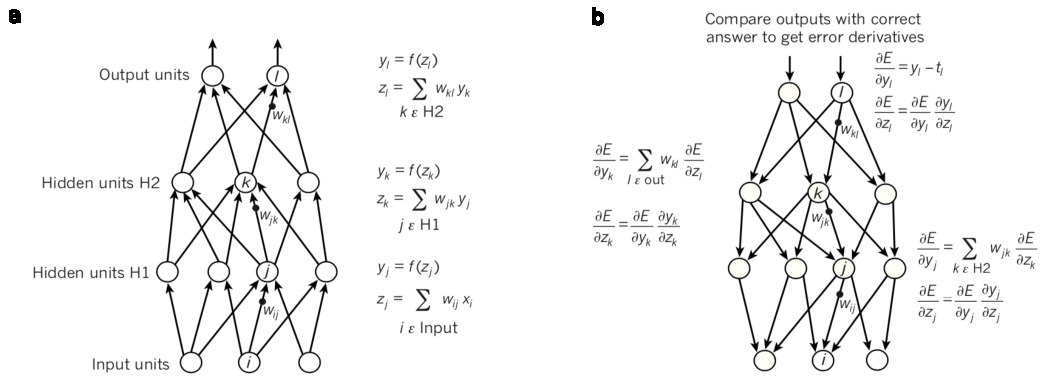
\includegraphics[width=1\textwidth]{Figures/simple_neural_net.pdf}
	\caption{\textbf{Example of 3-Layer Neural Network.} \textbf{(a)} Feed-forward representation of a neural network with two hidden units H1 and H2 and a binary output unit. The inputs to every layer are weighted averages, specified by the weights $w$, of the outputs of the previous layer. In every layer, the outputs are generated by applying a non-linear function to the inputs. The most popular function for this purpose is the ReLu (see text). \textbf{(b)} Back-propagation of the error in order to learn the optimal weights of the neural network. The error is quantified by a loss function $E$ at the output of the neural network, which is a measure of the discrepancy between the desired output and the actual output of the network. During backpropagation the chain-rule is applied recursively to the loss function in a backward manner. Specifically, at every layer the derivative of the error with respect to the inputs is computed by mutlipliying the upstream gradient with the local gradient. The upstream gradient is the derivative of the loss function with respect to the output of each unit, which is a weighted sum of the input derivatives of the layer above. The local gradient is the derivative of the non-linear function $f(z)$ with respect to its inputs. Starting from the output of the network one finally obtains the derivative of the loss function with respect to all weights, so that the network can minimze the loss by adjusting the weights. Panel is adapted from \parencite{lecun2015}.}
	\label{fig:simple_neural_net}
\end{figure}

As all machine learning models, deep learning models are trained by minimizing an objective function, i.e. by finding the optimal set of weights that achieve a specific input-output mapping. The minimization of the objective function is accomplished by applying gradient descent based methods, in practice, often  stochastic gradient descent \parencite{bottou2008} or variants of it \parencite{diederik2015}. The computation of the gradient of the objective function with respect to all weights of the network is accomplished using backpropagation \parencite{rumelhart1986} (see Fig.~\ref{fig:simple_neural_net}(b)).
Intuitively, the backpropagation algorithm helps to quantify the influence of every weight of the network on the final error, so that one can decrease the error by updating the weights in the direction of the negative gradient. \textcolor{red}{MENTION LOSS FUNCTION, FOR INSTANCE SOFTMAX}

Although artifical neural networks have been known and studied since the 1950s, it was only understood in the 1980s that mutlitlayer networks could be trained by backpropagation and stochastic gradient descent \parencite{lecun1989}. However, until recently, neural networks were still ignored by the computer-vision and speech-recognition communities, because of the believe that the objective function would get trapped in local minima. 

The advent of several new methods and technologies shall prove wrong the scepticism towards feasibly training deep neural networks. A requirement to reliable train large neural networks is the availability of large amounts of labelled data, as well as the necessary processing power. Both became available with the emergence of "Big Data" and new powerful graphics processing units (GPUs) about a decade ago.
Also theoretical advances helped to eliviate the difficulties to train deep learning models. These include the application of the ReLU non-linearity \parencite{glorot2011}, which solved the vanishing gradient problem, as well as the development of a particular type of NNs, the convolutional neural networks. These networks are much easier to train than conventional FC networks, have less parameters, and they generalize better to unseen data. 

\section{Convolutional Neural Networks}
Convolutional neural networks \parencite{vaillant1993, lecun1998} are specifically designed to process input data that has the shape of multiple arrays, such as the pixel values of a 2-dimensional image with three color channels. This is accomplished by using additional layers to preserve spatial structure. In general, a CNN is composed of several convolutional layers followed by a nonlinearity. These are often followed by a pooling layer, and a fully connected layer is used as the last layer of the network. The architecture of a small VGG convolutional net \parencite{simonyan2014}  used for classification is shown in Fig.~\ref{fig:convnet}.

With this design, CNNs take advantage of the natural properties of images. The central element here is the convolutional layer, which takes into account that local pixel values are highly correlated, and that the local statistics of images are invariant to translation \parencite{lawrence1997}. In particular, in a convolutional layer several small filters are slided spatially over the image computing dot products at every spatial location. The filters always extend the full depth of the input volume. For instance, a typical filter for a 3 color channel image might have dimensions $5 \times 5 \times 3$. Sliding this filter over an image of size, say  $32\times32\times3$, would lead to an activation map with dimensions $28\times28\times1$. 

The activation map is produced with one set of weights that belong to this particular filter. This concept is referred to as shared weights, which means that a comparatively small number of weights is shared across the entire image. As it is the case with conventional neural networks the weights, or parameters, are learned by applying gradient descent and backprogagation.  The number of weights, or parameters, per filter is given by the spatial filter size, times the depth of the image plus a bias term. In the usual case of multiple filters the number of parameters is multiplied by K, which corresponds to having K activation maps. Typically many filters are applied at every convolutional layer, so that every filter learns a set of weights that relate to one particular feature in the image (see Fig.~\ref{fig:convnet}(a)). 


\begin{figure}[h!]
	\centering
	\captionsetup{width=1\linewidth}
	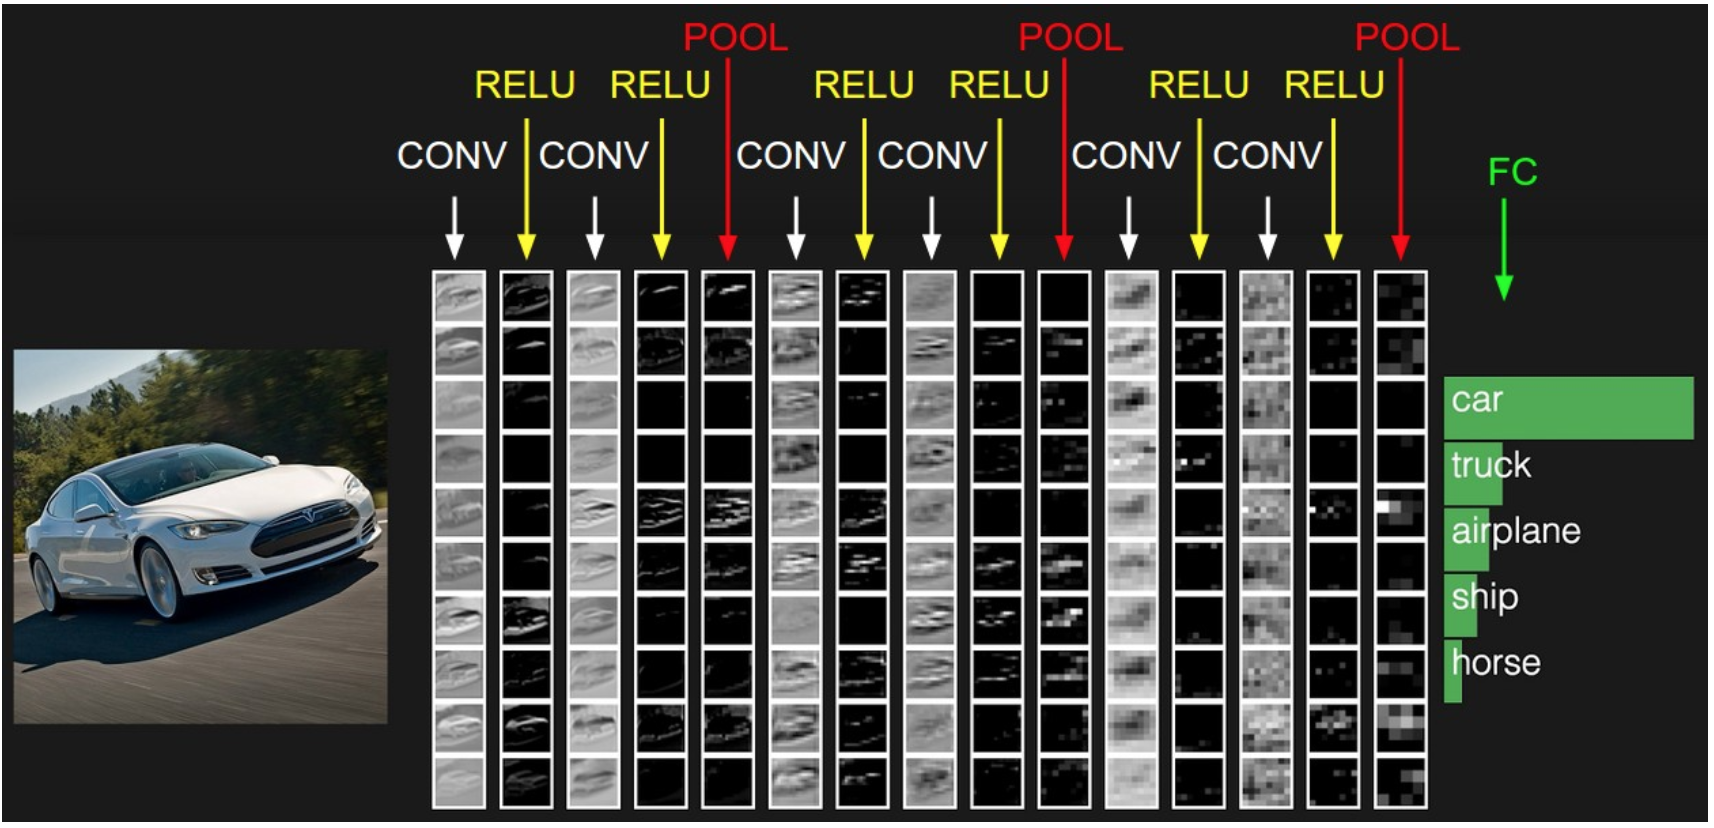
\includegraphics[width=0.8\textwidth]{Figures/convnet.png}
	\caption{\textbf{Activations of a convolutional neural network used for classification.} The forward pass in this network is computed from left to right. Every column represents a layer of the network and the small images are the filter activations when passing the passing the image through the network. The structure shown here is typical for CNNs in that it has convolutional layers followed by a non-linear activation function. Multiple layers of these are followed by a pooling layer. The output of the network are a set of class scores produced by the final fully connected layer. Figure is adapted from \parencite{cs231_convnets}.}
	\label{fig:convnet}
\end{figure}

The dimensions of the output of every convolutional layer are controlled by three parameters: the stride S, zero-padding P, and the number of filters with size F. The stride is the interval at which the filter is slided over the image. Zero-padding has the porpuse to increase the image size by adding pixels with zero value at the border, so that the input and output dimensions can be matched (assuming stride is 1). For an input image of size W the output activation map will have
\begin{equation}
\frac{W - F +2P}{S} + 1
\end{equation}
pixels along every dimension. 

\begin{figure}[h!]
	\centering
	\captionsetup{width=1\linewidth}
	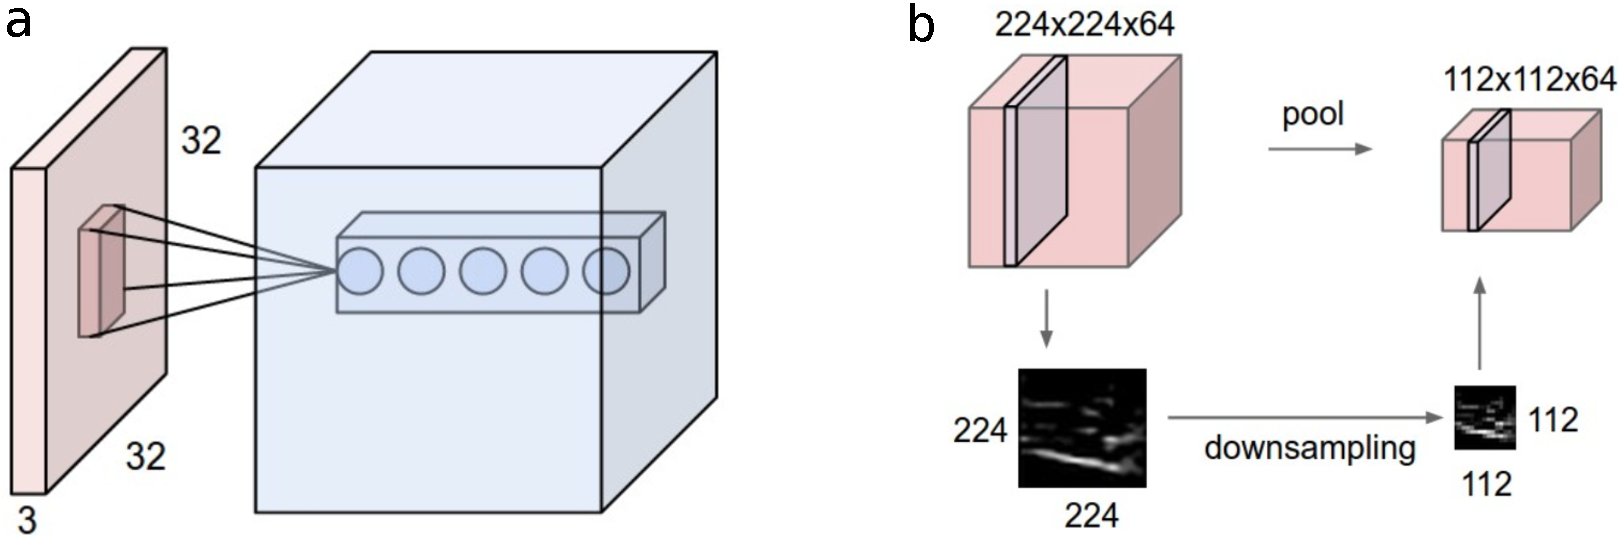
\includegraphics[width=0.85\textwidth]{Figures/conv_pooling.pdf}
	\caption{\textbf{Example of a convolutional layer (a) and a pooling layer (b).} \textbf{(a)} In this example a five small filter (represented by the 5 dots in the output volume) are applied to the input image of dimensions $32\times32\times3$. The filters extend over the entire input depth, but look only at a small region spatially, defined by the filter size. Every layer, i.e. every activation map in the output volume is generated by sliding one filter over the entire image. In essence, every filter is sensitive to a specific feature in the input image. \textbf{(b)} Schematic representation of the effect of a max-pooling layer with stride 2. Effectively the image is downsampled where in every 2-by-2 area of the input volume the maximum pixel value is passed to the output. Apart from downsampling, pooling introduces a invariance to local variations. Figure is adapted from \parencite{cs231}.
}
	\label{fig:conv_pooling}
\end{figure}

Pooling layers introduce coarse-graining in order to create invariance to small shifts and to decrease the number of parameters, which makes the representations smaller and more manageable. A pooling layer is applied to every activation map independently. It downsamples its input, in the most common case, by applying a max operator. This is shown schematically in Fig.~\ref{fig:conv_pooling}(b). Max-pooling with stride 2 would, for instance, transform a $4 \times 4$ input image to a $2 \times 2$ output image by taking the maximum element at every 2-by-2 location. Note that pooling layers don't have any parameters.

When stacking together mutliple combinations of convolutional layers followed by non-linearities and pooling layers, the filters learn a hierarchichal structure. The filters at earlier layers learn simple low-level features such as edges whereas the filters at later stages learn more complex high-level features, which are compositions of lower level features. In conclusion, the deeper a convolutional neural network is the more complex compositions of features it can learn.

\section{CNN Architectures}\label{sec:CNNArchitectures}
The AlexNet was the first convolutional neural network that achieved remarkable results in the ImageNet classification task in 2012. It halfed the error in comparison to all competing non deep learning based approaches (see Fig.~\ref{fig:imagenet}). In this competition deep convolutional networks were applied to a dataset with roughly 1 million images and 1000 classes. AlexNet was specifically designed to be trained on two GPUs with each 3GB of memory, which was sufficient to fit all the 60 million parameters inside. AlexNet had 8 layers, and used dropout as regularization technique.

\begin{figure}[h!]
	\centering
	\captionsetup{width=1\linewidth}
	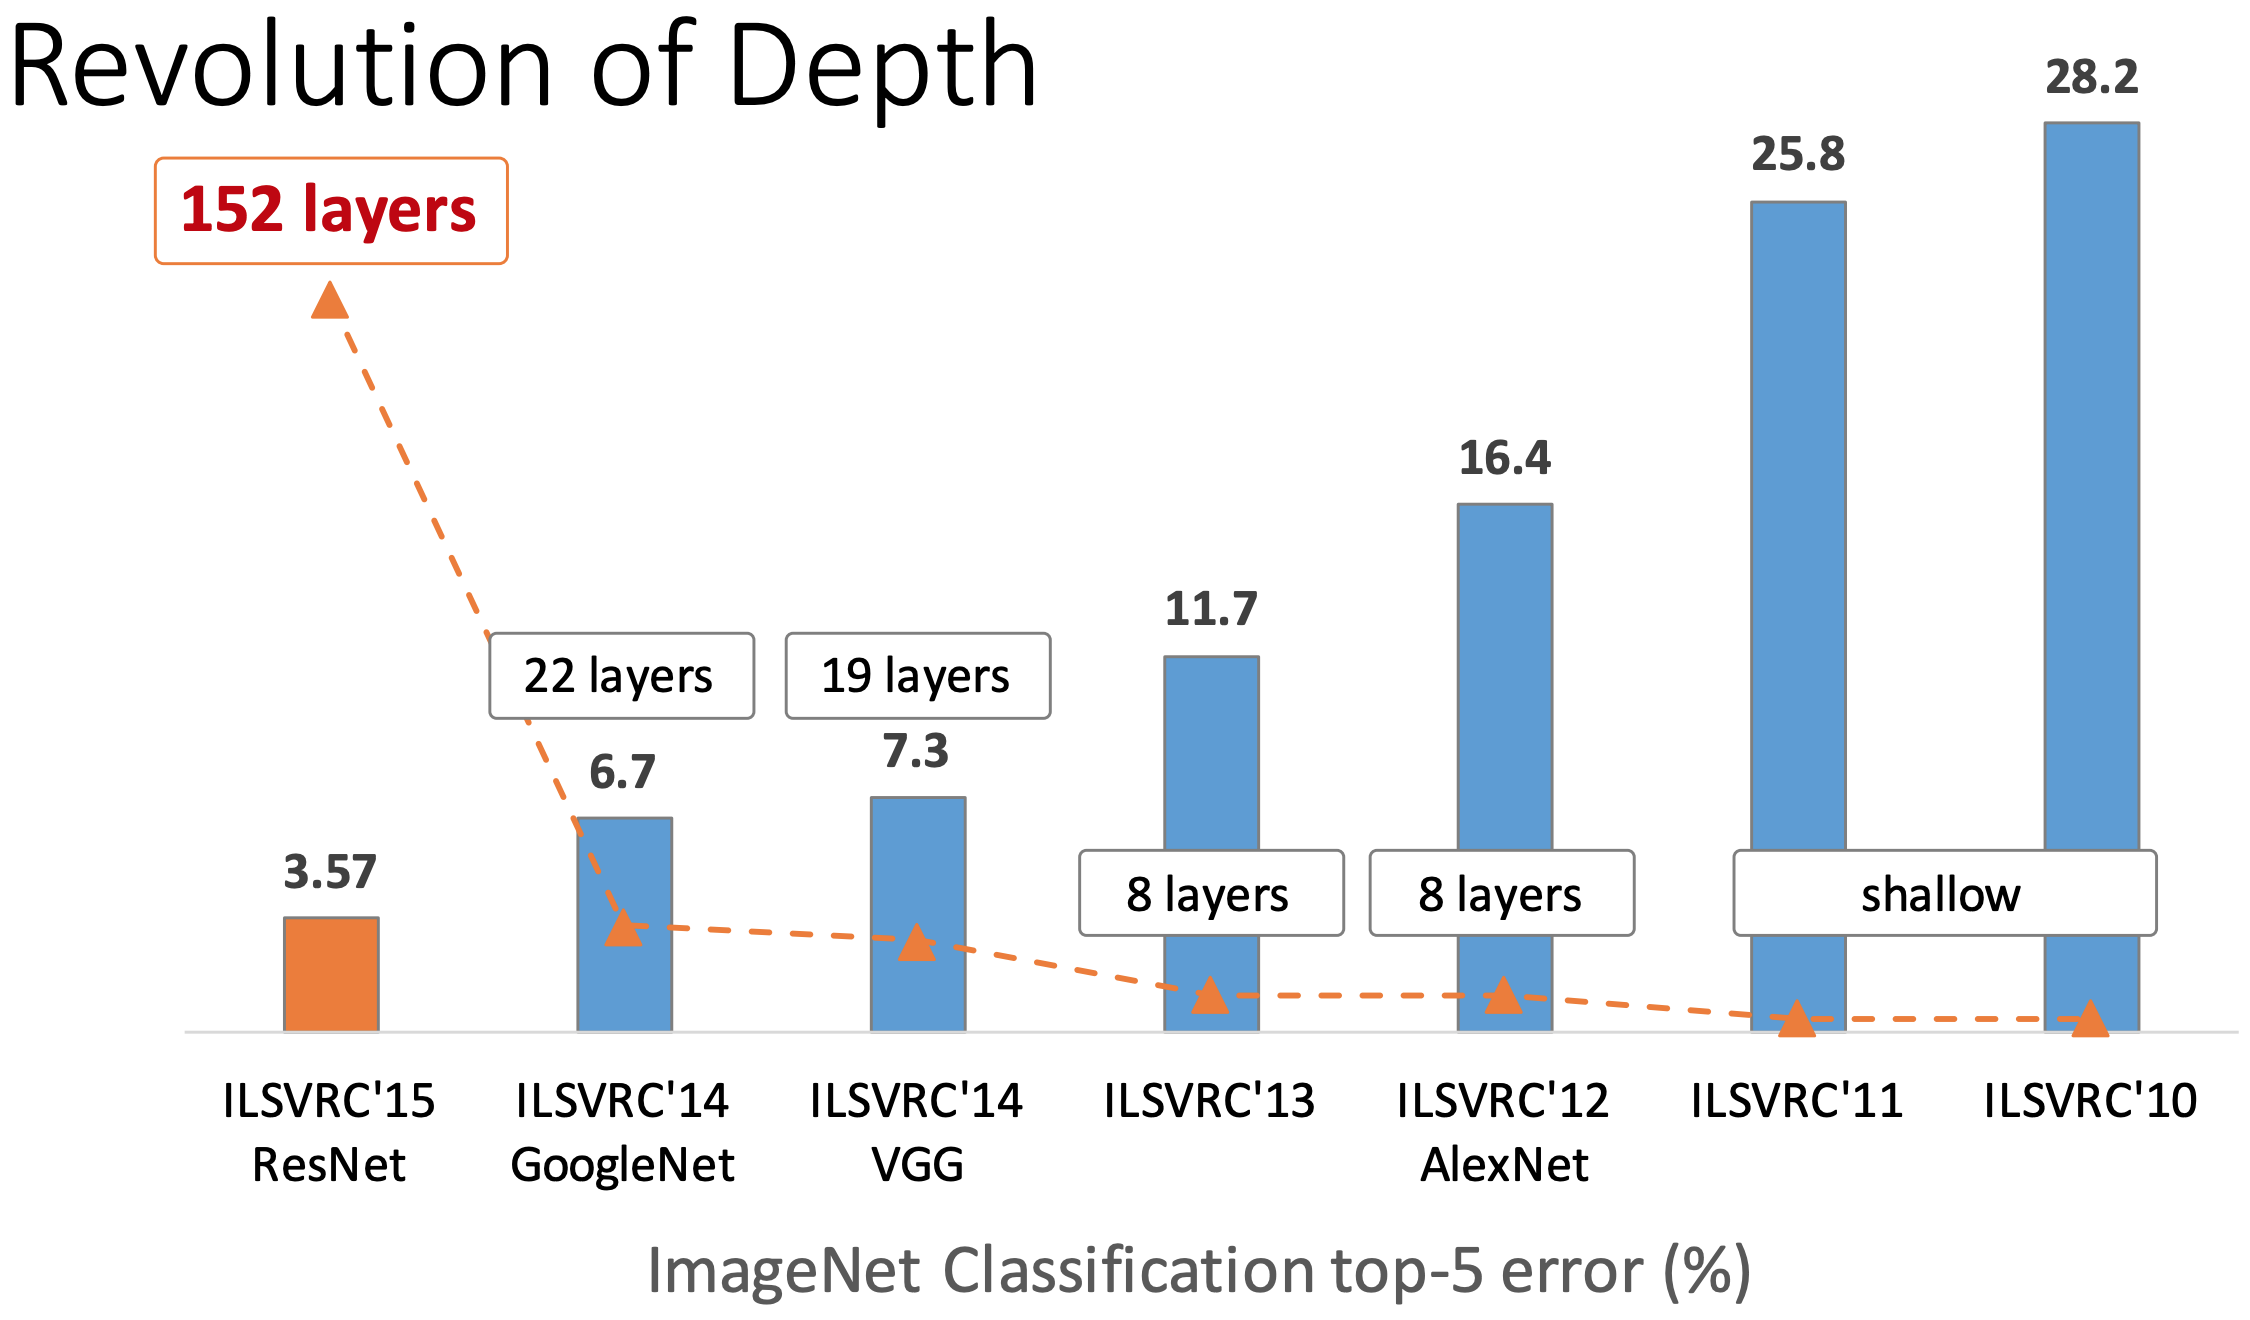
\includegraphics[width=0.85\textwidth]{Figures/imagenet_evolution.png}
	\caption{Top-5 test error of the winning solutions of the Large Scale Visual Recognition Challenge through years 2010 to 2015. Figure is adapted from this  \href{http://kaiminghe.com/icml16tutorial/icml2016_tutorial_deep_residual_networks_kaiminghe.pdf}{link}.}
	\label{fig:imagenet}
\end{figure}

The winner of the ILSVRC2013 was the ZFNet \parencite{zeiler2013}, which basically had improved hyperparameters compared to the AlexNet. In 2014, two networks were developed that were significantly deeper than previous networks. The VGG network \parencite{simonyan2014} had 19 layers and the GoogleNet had 22 layers \parencite{szegedy2014}. To be able to increase the number of layers, researchers from Oxford used very small filters ($3\times3$) in VGG thereby reducing the number of parameters per layer significantly. The GoogleNet first introduced the Inception module, which is used 9 times.The idea behind the Inception module is to have several small networks within the network that do multiple convolutions and pooling in parallel. In combination with getting rid of fully connected layers, the GoogleNet has only 5 million parameters, 12 times less than the AlexNet. 

The researchers that developed ResNet \parencite{he2015}, which was the ImageNet classification winner in 2015, wanted to answer the question: What happens when we continue stacking deeper layers on a plain convolutional network? By comparing a 20 layer network with a 56 layer network they found, that the deeper network had lower performance both on the training set and on the test set. This implies that there is a fundamental problem, since overfitting can be excluded. The authors hypothesized that the origin of this observation must have it's roots in wrong optimisation of the objective function. The argument they gave was that a deeper network always must perform at least as good as a shallower network. This can be seen when one replaces some of the modules in the deeper network by identity mappings. \textcolor{red}{REWRITE THIS PARAGRAPH TO BE MORE COMPACT, AND MORE PRECISE.}

\begin{figure}[h!]
	\centering
	\captionsetup{width=1\linewidth}
	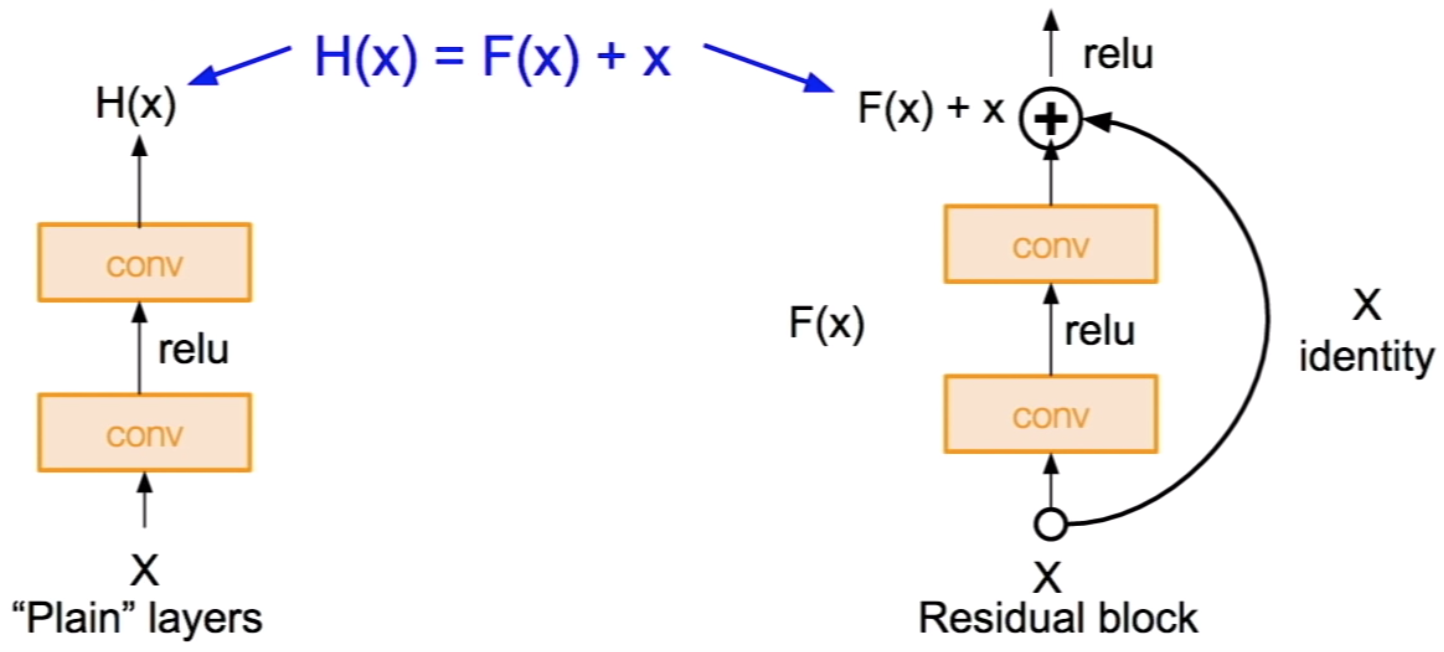
\includegraphics[width=0.7\textwidth]{Figures/residual_modul.png}
	\caption{\textbf{Residual block of ResNet architecture.} Comparison between plain convolutional architecture (left) and convolutional architecture using a residual block. For the plain structure the network learns the mapping $H(x)$ while for the residual structure the network learns a residual $F(x) = H(x) - x$. x here is the identity mapping. Figure is adapted from \parencite{cs231}.}
	\label{fig:residual}
\end{figure}

So instead of simply stacking more and more layers together He et al. developed residual blocks containing an identity mapping additionally to the convolutional layer. When having an identity mapping between input and output the network just needs to learn the residual connections represented as $F(x)$ in Fig.~\ref{fig:resnet}.
Taking advantage of this approach they were able to design networks with a depth of up to 152 layers, which allowed for halfing the error rate of the ImageNet dataset in the year 2015. 

\begin{figure}[h!]
	\centering
	\captionsetup{width=1\linewidth}
	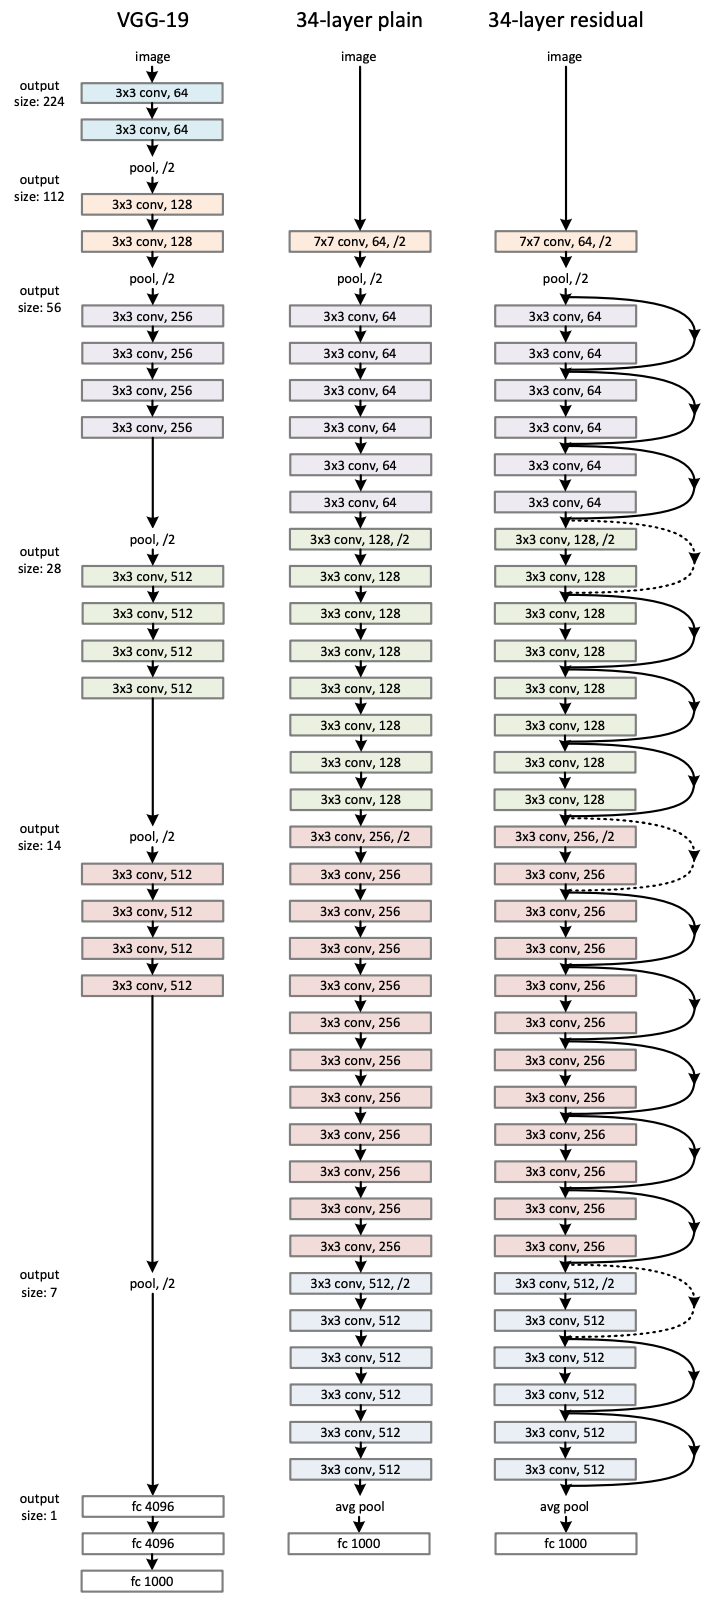
\includegraphics[width=0.6\textwidth]{Figures/resnet_architecture.png}
	\caption{\textbf{Comparison between deep convolutional neural network architectures.} On the left we have a VGG network with 19 layers, in the center a plain ResNet with 34 layers, and on the right a ResNet with 34 layers and residual connections. Figure is adapted from\parencite{he2015}.}
	\label{fig:resnet}
\end{figure}

The architecture of a ResNet with 34 layers is shown in Fig.~\ref{fig:resnet}. The first convolutional layer has a filter size of $7\times7$ while all consecutive filters are chosen to be as small as possible ($3\times$). After every convolutional block that contains mutliple convolutional layers and residual blocks the image is downsampled with stride 2 and the number of filters is doubled, so that effectively the spatial size decreases while the depth increases. The network is terminated with an average pooling layer, and a 1000 fully connected layer for the 1000 classes of the ImageNet dataset. Overall, He and coworkers constructed ResNet architectures with 34, 50, 101, and 152 layers.

After the ResNet several other networks have been developed, but they only performed incrementally better and most of them were more sophisticated versions of the ResNet or combinations of the ResNet with other architectures, such as Inception-V4 \parencite{szegedy2016}. We therefore decided to use a ResNet architecture that was pretrained on ImageNet for the experiment in this thesis. \textcolor{red}{MENTION: FRACTAL NET AND LAYER DROPOUT, DENSENT.}
